\documentclass[letter,11pt]{article}

\usepackage[spanish,es-nodecimaldot]{babel}
\usepackage[utf8]{inputenc}

\usepackage{lmodern}
\usepackage[T1]{fontenc}
\usepackage{textcomp}

\usepackage{framed}
\usepackage[svgnames]{xcolor}
\colorlet{shadecolor}{Gainsboro!50}

\usepackage[labelfont=bf]{caption}
\usepackage{graphicx}
\usepackage{pstricks}
\usepackage{amsmath}

\usepackage{anysize}
\marginsize{3cm}{2cm}{2cm}{3cm}

\usepackage{fancyhdr}
\usepackage{lastpage}
\pagestyle{fancy}
\fancyhf{}
\fancyhead[LE,RO]{Momento de Inercia}
\fancyfoot[CO,CE]{\thepage\ de \pageref{LastPage}}

\special{papersize=215.9mm,279.4mm}

\usepackage[
    pdfauthor={Carlos Eduardo Caballero Burgoa},%
    pdftitle={Física Básica II},%
    pdfsubject={Momento de Inercia},%
    colorlinks,%
    citecolor=black,%
    filecolor=black,%
    linkcolor=black,%
    urlcolor=black,
    breaklinks]{hyperref}
\usepackage{breakurl}

\begin{document}

\begin{titlepage}
\begin{center}
{\Large UNIVERSIDAD MAYOR DE SAN SIMÓN}\\
\vspace*{0.15cm}
{\large FACULTAD DE CIENCIAS Y TECNOLOGÍA}\\
\vspace*{0.10cm}
DEPARTAMENTO DE FÍSICA\\
\vspace*{3.0cm}
{\Large \textbf{FÍSICA BÁSICA II}}\\
\vspace*{0.3cm}
{\Large \textbf{Tarea de Investigación}}\\
\vspace*{3.5cm}
{\Large \textbf{MOMENTO DE INERCIA}}\\
\end{center}

\vspace*{7.8cm}
\leftskip=7.95cm
\noindent
\textbf{Estudiante:}\\
Caballero Burgoa, Carlos Eduardo.\\
\newline
\textbf{Docente:}\\
Ing. Moreira Calizaya, Rene.\\
\newline
\textbf{Grupo:} J.\\
\textbf{Fecha de entrega:} 30 de Abril del 2021.\\

\end{titlepage}

\section{Introducción}
Cuando se analiza un movimiento traslacional y rectilíneo se considera a la masa
del objeto como una medida de su inercia. Por lo tanto, la masa es una medida de
la inercia de un cuerpo y es en este sentido, una medida de su resistencia al
cambio de velocidad.

Análogamente, al hacer que un objeto sólido rote o se mueva en trayectoria
curva, se observa una resistencia al cambio del movimiento rotacional. Esta
oposición del objeto al cambio de su rotación se conoce como inercia rotacional
o \textbf{momento de inercia}. En otras palabras, en el movimiento circular el
momento de inercia cumple el mismo rol que la masa juega en el movimiento
rectilíneo \cite{FISIC.CH}.

\section{Sistema de partículas\cite{Sears}}
Se tiene un cuerpo formado por un sistema de partículas (véase la \textbf{Figura
\ref{figura1}}), con masas $m_1$, $m_2$, $m_3$, ..., $m_i$, ..., $m_{n-1}$,
$m_n$, a distancias perpendiculares $r_1$, $r_2$, $r_3$, ..., $r_i$, ...,
$r_{n-1}$, $r_n$ del eje de rotación.

\begin{figure}
\centering
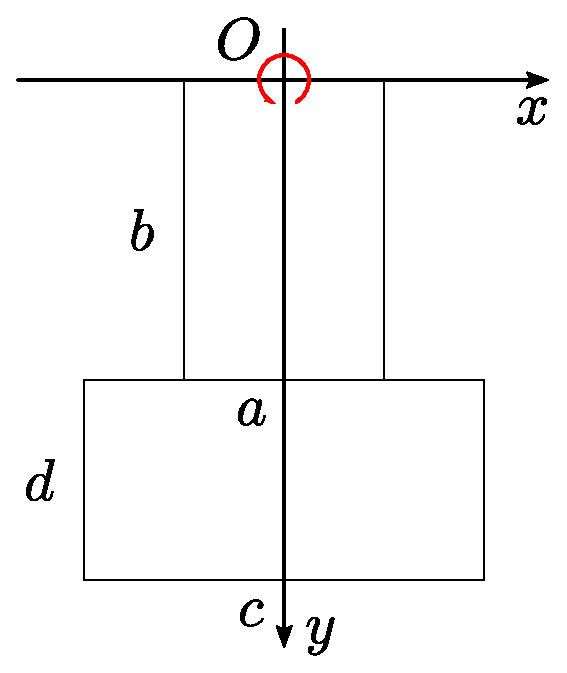
\includegraphics[width=0.42\textwidth]{resources/f1.eps}
\caption{Sistema de partículas girando alrededor de un eje.}
\label{figura1}
\end{figure}

Cuando este sistema de partículas gira alrededor de un eje fijo, la rapidez
$v_i$ de cada partícula esta dada por:

\begin{equation*}
    v = r \omega
\label{velocidad}
\end{equation*}

Donde $\omega$ es la magnitud de la velocidad angular del sistema de partículas
medida en $rad/s$. Cada partícula tiene un $r_i$ diferente, pero todas comparten
el mismo valor de $\omega$ (si es que consideramos el sistema de partículas como
un cuerpo rígido), por tanto la energía cinética de cada partícula es:

\begin{equation*}
    \frac{1}{2} m_i v^2_i = \frac{1}{2} m_i r^2_i \omega^2
\label{cinetica}
\end{equation*}

La energía cinética total del sistema de partículas es la suma de las energías
cinéticas de todas sus partículas:

\begin{equation*}
    K = \frac{1}{2} m_1 r^2_1 \omega^2 + ... + \frac{1}{2} m_n r^2_n \omega^2 = \sum_{i=1}^{n} \frac{1}{2} m_i r^2_i \omega^2
\label{cineticatotal1}
\end{equation*}

Sacando el factor común $\omega^2/2$ de la expresión, se obtiene:

\begin{equation*}
    K = \frac{1}{2} (m_1 r^2_1 + ... + m_n r^2_n ) \omega^2 = \frac{1}{2} \left( \sum_{i=1}^{n} m_i r^2_i \right) \omega^2
\label{cineticatotal2}
\end{equation*}

La cantidad entre paréntesis, que se obtiene multiplicando la masa de cada
partícula por el cuadrado de su distancia al eje de rotación y sumando los
productos, se denota con $I$, y es el \textbf{momento de inercia} del cuerpo
para este eje de rotación:

\begin{equation}
    I = m_1 r^2_1 + ... + m_n r^2_n = \sum_{i=1}^{n} m_i r^2_i
\label{momentodeinercia}
\end{equation}

Para un cuerpo con un eje de rotación dado y una masa total determinada, cuanto
mayor sea la distancia del eje a las partículas que constituyen el cuerpo, mayor
será el momento de inercia.

En términos del momento de inercia $I$, la \textbf{energía cinética de rotación}
$K$ de un cuerpo rígido es:

\begin{equation}
    K = \frac{1}{2} I \omega^2
\label{cineticarotacional}
\end{equation}

Entonces, cuanto mayor sea el momento de inercia, mayor será la energía cinética
de un cuerpo rígido que gira con una rapidez angular $\omega$. Y sabiendo que la
energía cinética de un cuerpo es igual al trabajo efectuado para acelerar ese
cuerpo desde el reposo, podemos asumir que cuanto mayor sea el momento de
inercia de un cuerpo, más difícil sera ponerlo a girar si está en reposo, y más
difícil será detener su rotación si ya está girando.

\vspace{0.75cm}
\begin{minipage}[b]{.4\linewidth}
\textbf{Ejemplo 1}:\\
Se tiene un sistema de 6 partículas como se muestra en la figura. \\

a) Calcular el momento de inercia del sistema para el eje de rotación $y = 6$, \\
b) Calcular la energía cinética rotacional si el sistema gira con una rapidez
angular $\omega = 4.0 [rad/s]$.
\end{minipage}\hfill
\begin{minipage}{.5\linewidth}
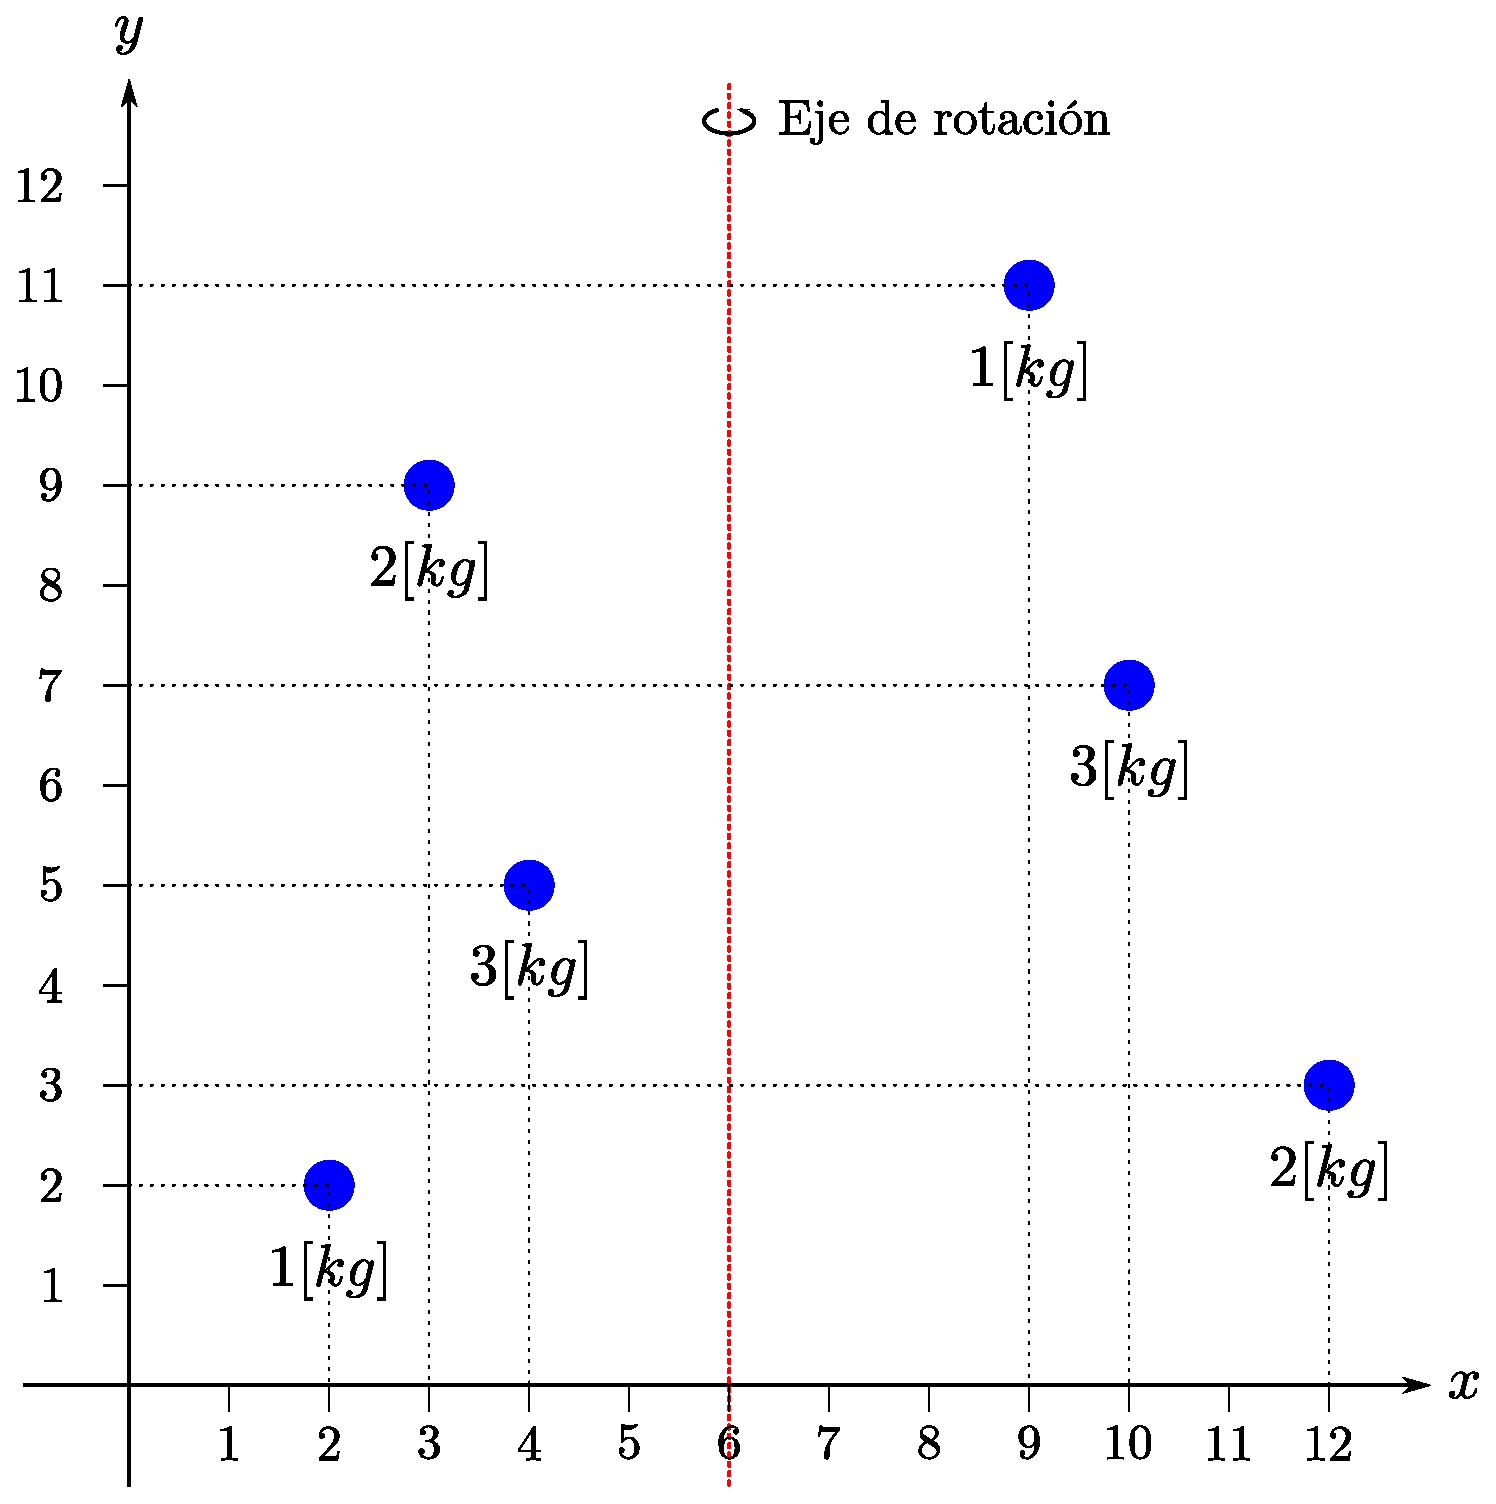
\includegraphics[width=0.95\textwidth]{resources/f2.eps}
\end{minipage}

\begin{minipage}[b]{.9\linewidth}
\textbf{Solución}:\\
a) Para calcular el momento de inercia se utilizara la \textbf{ecuación
(\ref{momentodeinercia})}, y se calculará la distancia perpendicular
aprovechando que el eje es vertical.

\begin{equation*}
    I = \sum_{i=1}^{6} m_i r^2_i = 1 (4)^2 + 2(3)^2 + 3(2)^2 + 1(3)^2 + 3(4)^2 + 2(6)^2 = 175 [kg\, m^2]
\end{equation*}

b) Una vez calculado el momento de inercia para el eje propuesto, se puede
calcular la energía cinética con la \textbf{ecuación
(\ref{cineticarotacional})}:

\begin{equation*}
    K = \frac{1}{2} I \omega^2 =  \frac{1}{2} \left(175 [kg\, m^2]\right) \left(4.0 \left[\frac{rad}{s^2}\right]\right) = 350 [J]
\end{equation*}
\end{minipage}

\vspace{0.75cm}
\begin{minipage}[b]{.4\linewidth}
\textbf{Ejemplo 2}:\\
Se tiene el sistema de 6 partículas anteriormente citado como se muestra en la
figura. \\

a) Calcular el momento de inercia del sistema para el eje de rotación $y = x$, \\
b) Calcular la energía cinética rotacional si el sistema gira con una rapidez
angular $\omega = 4.0 [rad/s]$.
\end{minipage}\hfill
\begin{minipage}{.5\linewidth}
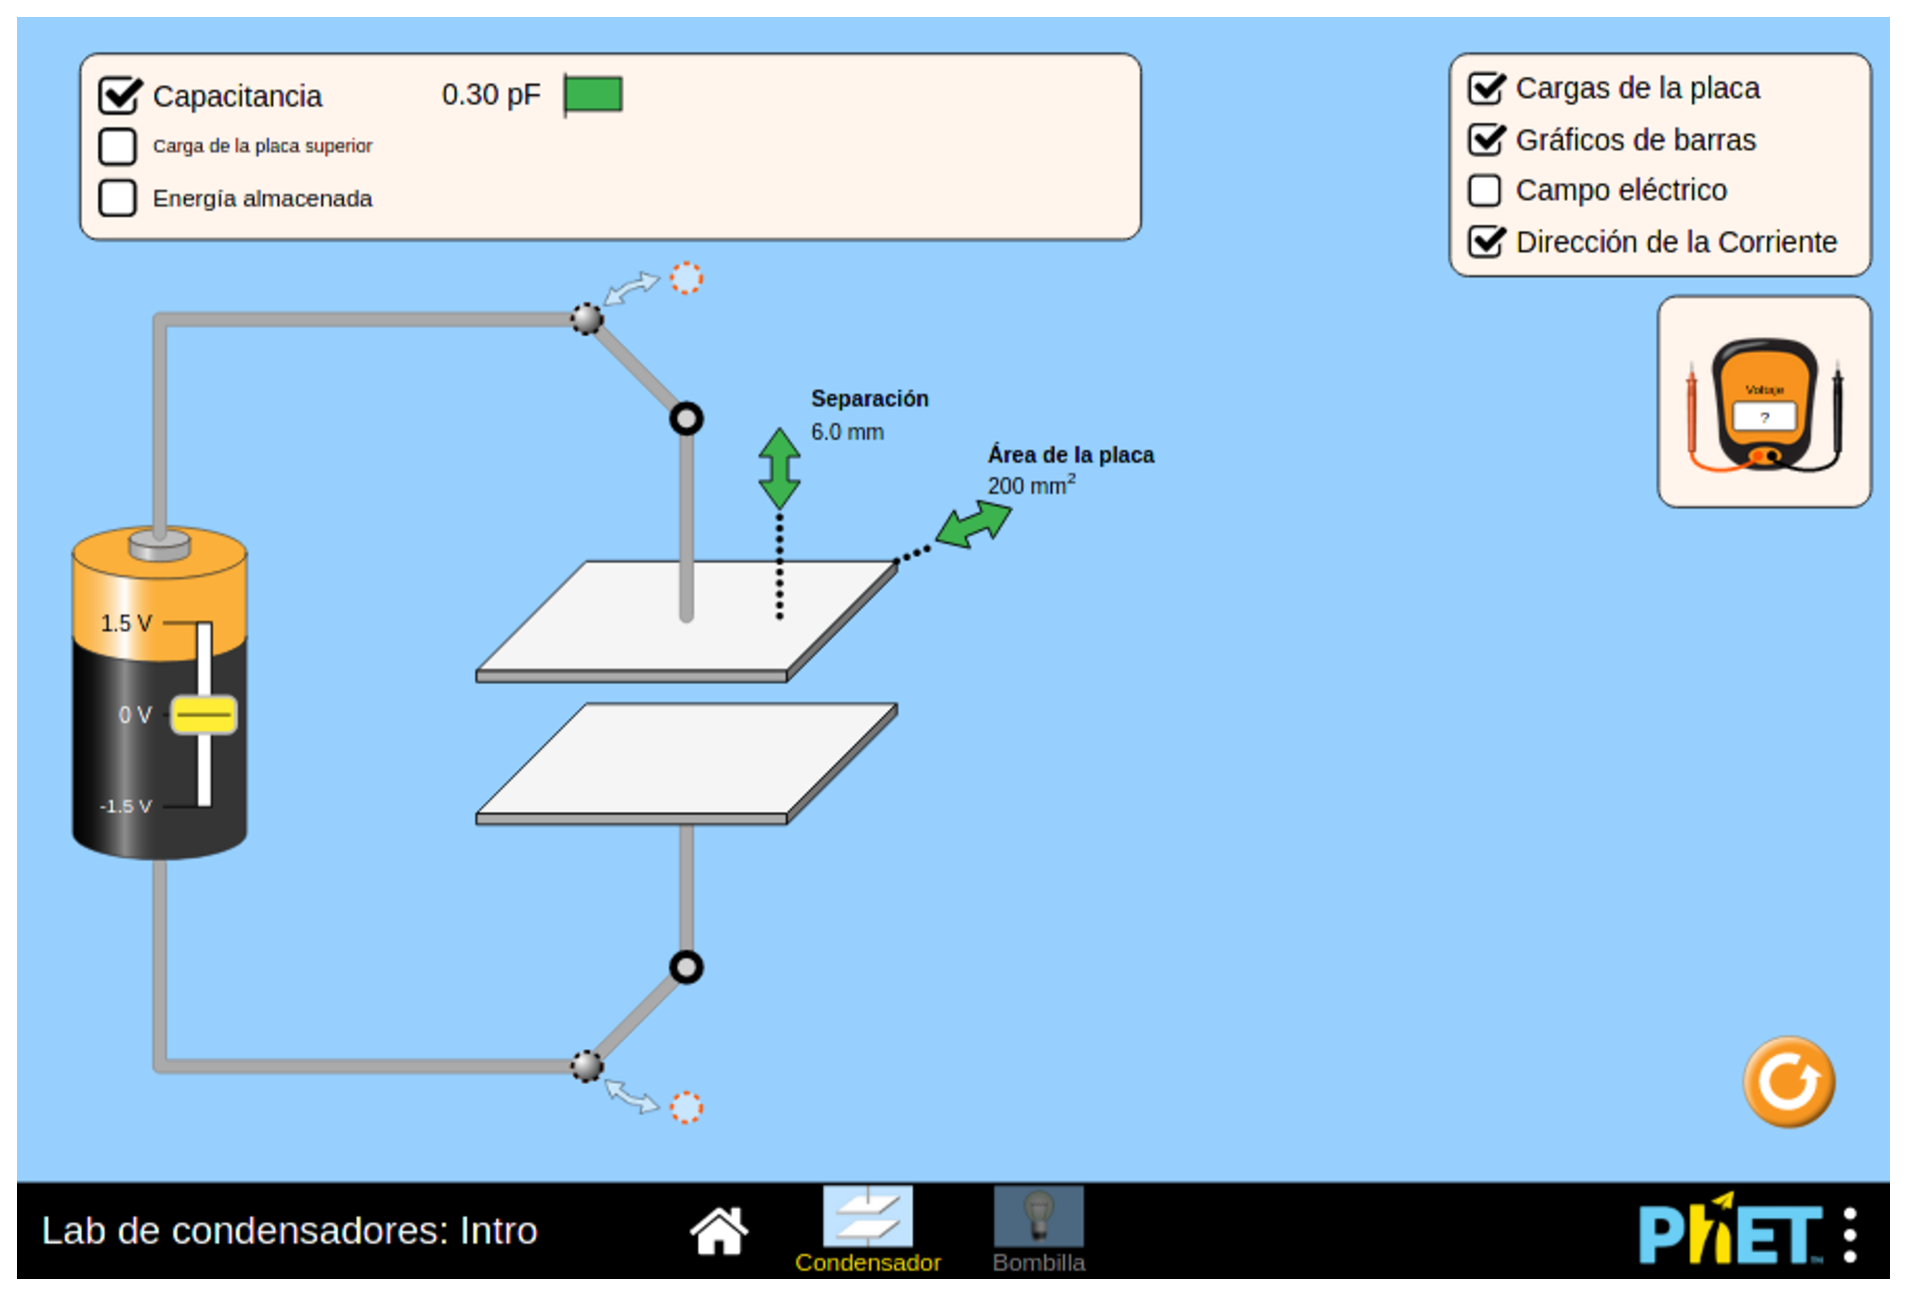
\includegraphics[width=0.95\textwidth]{resources/f3.eps}
\end{minipage}

\vspace{0.50cm}
\begin{minipage}[b]{.9\linewidth}
\textbf{Solución}:\\
a) Para calcular el momento de inercia se utilizará la \textbf{ecuación
(\ref{momentodeinercia})}, y considerando que el eje es diagonal al sistema de
referencia, se debe calcular la distancia perpendicular a tal eje:

Ecuación de la recta:
\begin{equation*}
    x - y = 0
\end{equation*}

Distancia de una recta a un punto:
\begin{equation*}
    d = \frac{| A x + B y + C |}{\sqrt{A^2 + B^2}}
\end{equation*}

Por tanto:
\begin{equation*}
    d_1(2,2) = \frac{| 1 (2) - 1 (2) |}{\sqrt{1^2 + (-1)^2}} = \frac{|2 - 2|}{\sqrt{2}} = 0
\end{equation*}
\begin{equation*}
    d_2(3,9) = \frac{| 1 (3) - 1 (9) |}{\sqrt{1^2 + (-1)^2}} = \frac{|3 - 9|}{\sqrt{2}} = \frac{6}{\sqrt{2}}
\end{equation*}
\end{minipage}

\begin{minipage}[b]{.9\linewidth}
\begin{equation*}
    d_3(4,2) = \frac{| 1 (4) - 1 (2) |}{\sqrt{1^2 + (-1)^2}} = \frac{|4 - 2|}{\sqrt{2}} = \frac{2}{\sqrt{2}}
\end{equation*}
\begin{equation*}
    d_4(9,11) = \frac{| 1 (9) - 1 (11) |}{\sqrt{1^2 + (-1)^2}} = \frac{|9 - 11|}{\sqrt{2}} = \frac{2}{\sqrt{2}}
\end{equation*}
\begin{equation*}
    d_5(10,7) = \frac{| 1 (10) - 1 (7) |}{\sqrt{1^2 + (-1)^2}} = \frac{|10 - 7|}{\sqrt{2}} = \frac{3}{\sqrt{2}}
\end{equation*}
\begin{equation*}
    d_6(12,3) = \frac{| 1 (12) - 1 (3) |}{\sqrt{1^2 + (-1)^2}} = \frac{|12 - 3|}{\sqrt{2}} = \frac{9}{\sqrt{2}}
\end{equation*}

\begin{equation*}
    I = \sum_{i=1}^{6} m_i r^2_i = 1 (0) + 2\left(\frac{6}{\sqrt{2}}\right)^2 + 3\left(\frac{2}{\sqrt{2}}\right)^2 + 1\left(\frac{2}{\sqrt{2}}\right)^2 + 3\left(\frac{3}{\sqrt{2}}\right)^2 + 2\left(\frac{9}{\sqrt{2}}\right)^2
\end{equation*}
\begin{equation*}
    I = 2 \left(\frac{36}{2}\right) + 3 \left(\frac{4}{2}\right) + 1 \left(\frac{4}{2}\right) + 3 \left(\frac{9}{2}\right) + 2 \left(\frac{81}{2}\right) = \frac{277}{2} [kg\, m^2]
\end{equation*}

b) Una vez calculado el momento de inercia para el eje propuesto, se puede
calcular la energía cinética con la \textbf{ecuación
(\ref{cineticarotacional})}:

\begin{equation*}
    K = \frac{1}{2} I \omega^2 =  \frac{1}{2} \left(\frac{277}{2} [kg\, m^2]\right) \left(4.0 \left[\frac{rad}{s^2}\right]\right) = 277 [J]
\end{equation*}
\end{minipage}

\vspace{0.75cm}
\begin{minipage}[c]{.4\linewidth}
\textbf{Ejemplo 3}:\\
Se tiene el sistema de 4 partículas como se muestra en la figura cuyas masas y
posiciones son:

\begin{equation*}
    m_1 = 1 [kg]\; p_1 = (2,5,3)
\end{equation*}
\begin{equation*}
    m_2 = 2 [kg]\; p_2 = (6,0,0)
\end{equation*}
\begin{equation*}
    m_3 = 3 [kg]\; p_3 = (6,8,1)
\end{equation*}
\begin{equation*}
    m_4 = 4 [kg]\; p_4 = (12,2,1)
\end{equation*}

a) Calcular el momento de inercia del sistema para el eje de rotación que pasa
por los puntos $A = (0,2,1)$ y $B = (12,11,5)$. \\
b) Calcular la energía cinética rotacional si el sistema gira con una rapidez
angular $\omega = 4.0 [rad/s]$.
\end{minipage}\hfill
\begin{minipage}{.5\linewidth}
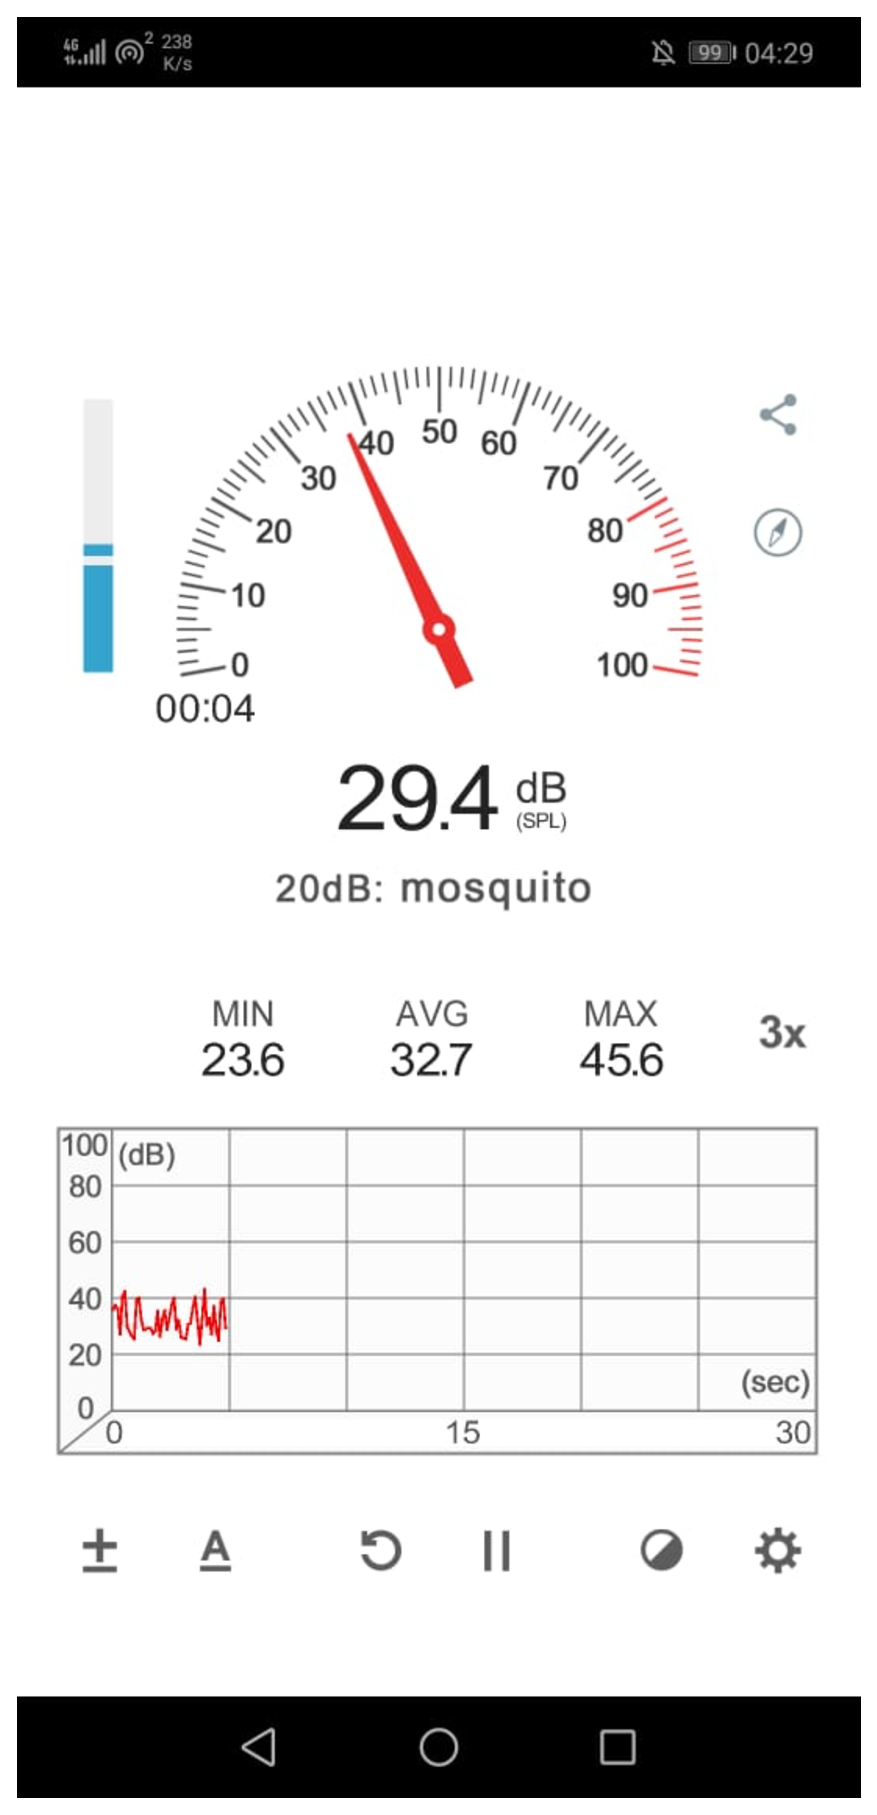
\includegraphics[width=0.95\textwidth]{resources/f4.eps}
\end{minipage}

\vspace{0.50cm}
\begin{minipage}[b]{.9\linewidth}
\textbf{Solución}:\\
a) Para calcular el momento de inercia se utilizará la \textbf{ecuación
(\ref{momentodeinercia})}, y se usaran operaciones vectoriales para facilitar el
trabajo con tres dimensiones:
Vector posición del eje:
\begin{equation*}
    \vec{r}_{AB} = B - A = (12,11,5) - (0,2,1) = (12,9,4)
\end{equation*}
\end{minipage}

\begin{minipage}[b]{.9\linewidth}
Distancia mínima de un punto $P_i$ a la linea de $A$ a $B$:
\begin{equation*}
    d = | \vec{r}_{AP_i} | \left(\frac{| \vec{r}_{AP_i} \times \vec{r}_{AB} |}{|\vec{r}_{AP_i}| |\vec{r}_{AB}|} \right)
\end{equation*}

Por tanto:
\begin{equation*}
    d_1(2,5,3) = |(2,3,2)| \left(\frac{|(2,3,2)\times(12,9,4)|}{|(2,3,2)||(12,9,4)|}\right) = 1.5988
\end{equation*}
\begin{equation*}
    d_2(6,0,0) = |(6,-2,-1)| \left(\frac{|(6,-2,-1)\times(12,9,4)|}{|(6,-2,-1)||(12,9,4)|}\right) = 5.5341
\end{equation*}
\begin{equation*} 
    d_3(6,8,1) = |(6,6,0)| \left(\frac{|(6,6,0)\times(12,9,4)|}{|(6,6,0)||(12,9,4)|}\right) = 2.4748
\end{equation*}
\begin{equation*}
    d_4(12,2,1) = |(12,0,0)| \left(\frac{|(12,0,0)\times(12,9,4)|}{|(12,0,0)||(12,9,4)|}\right) = 7.6130
\end{equation*}

\begin{equation*}
    I = \sum_{i=1}^{4} m_i r^2_i = 1 (1.5988)^2 + 2 (5.5341)^2 + 3 (2.4748)^2 + 4 (7.6130)^2 = 314.02 [kg\, m^2]
\end{equation*}

b) Una vez calculado el momento de inercia para el eje propuesto, se puede
calcular la energía cinética con la \textbf{ecuación
(\ref{cineticarotacional})}:

\begin{equation*}
    K = \frac{1}{2} I \omega^2 =  \frac{1}{2} (314.02 [kg\, m^2]) \left(4.0 \left[\frac{rad}{s^2}\right]\right) = 628.03 [J]
\end{equation*}
\end{minipage}


\section{Enunciado}





Realizar el desarrollo de la teoria y ejemplos de aplicacion de
momentos de inercia. Debe analizar los siguientes casos:
2. Sistema continuo de particulas (solido), analizando distribuciones de masa:
2.1 Lineal
2.2 Superficial
2.3 Volumétrica


\begin{thebibliography}{99}

\bibitem{FISIC.CH} Momento de Inercia \\
Extraído el 21 de Abril del 2021, de: \\
\url{https://www.fisic.ch/contenidos/din%C3%A1mica-rotacional/momento-de-inercia/}.
 
\bibitem{Sears} Sears y Zemansky (2013).\\
Física Universitaria. Volumen 1.\\
13va Edición.\\
Capitulo 9: Rotación de cuerpos rígidos.

\end{thebibliography}

\end{document}

